% Options for packages loaded elsewhere
\PassOptionsToPackage{unicode}{hyperref}
\PassOptionsToPackage{hyphens}{url}
%
\documentclass[
]{article}
\usepackage{amsmath,amssymb}
\usepackage{lmodern}
\usepackage{iftex}
\ifPDFTeX
  \usepackage[T1]{fontenc}
  \usepackage[utf8]{inputenc}
  \usepackage{textcomp} % provide euro and other symbols
\else % if luatex or xetex
  \usepackage{unicode-math}
  \defaultfontfeatures{Scale=MatchLowercase}
  \defaultfontfeatures[\rmfamily]{Ligatures=TeX,Scale=1}
\fi
% Use upquote if available, for straight quotes in verbatim environments
\IfFileExists{upquote.sty}{\usepackage{upquote}}{}
\IfFileExists{microtype.sty}{% use microtype if available
  \usepackage[]{microtype}
  \UseMicrotypeSet[protrusion]{basicmath} % disable protrusion for tt fonts
}{}
\makeatletter
\@ifundefined{KOMAClassName}{% if non-KOMA class
  \IfFileExists{parskip.sty}{%
    \usepackage{parskip}
  }{% else
    \setlength{\parindent}{0pt}
    \setlength{\parskip}{6pt plus 2pt minus 1pt}}
}{% if KOMA class
  \KOMAoptions{parskip=half}}
\makeatother
\usepackage{xcolor}
\usepackage[margin=1in]{geometry}
\usepackage{color}
\usepackage{fancyvrb}
\newcommand{\VerbBar}{|}
\newcommand{\VERB}{\Verb[commandchars=\\\{\}]}
\DefineVerbatimEnvironment{Highlighting}{Verbatim}{commandchars=\\\{\}}
% Add ',fontsize=\small' for more characters per line
\usepackage{framed}
\definecolor{shadecolor}{RGB}{248,248,248}
\newenvironment{Shaded}{\begin{snugshade}}{\end{snugshade}}
\newcommand{\AlertTok}[1]{\textcolor[rgb]{0.94,0.16,0.16}{#1}}
\newcommand{\AnnotationTok}[1]{\textcolor[rgb]{0.56,0.35,0.01}{\textbf{\textit{#1}}}}
\newcommand{\AttributeTok}[1]{\textcolor[rgb]{0.77,0.63,0.00}{#1}}
\newcommand{\BaseNTok}[1]{\textcolor[rgb]{0.00,0.00,0.81}{#1}}
\newcommand{\BuiltInTok}[1]{#1}
\newcommand{\CharTok}[1]{\textcolor[rgb]{0.31,0.60,0.02}{#1}}
\newcommand{\CommentTok}[1]{\textcolor[rgb]{0.56,0.35,0.01}{\textit{#1}}}
\newcommand{\CommentVarTok}[1]{\textcolor[rgb]{0.56,0.35,0.01}{\textbf{\textit{#1}}}}
\newcommand{\ConstantTok}[1]{\textcolor[rgb]{0.00,0.00,0.00}{#1}}
\newcommand{\ControlFlowTok}[1]{\textcolor[rgb]{0.13,0.29,0.53}{\textbf{#1}}}
\newcommand{\DataTypeTok}[1]{\textcolor[rgb]{0.13,0.29,0.53}{#1}}
\newcommand{\DecValTok}[1]{\textcolor[rgb]{0.00,0.00,0.81}{#1}}
\newcommand{\DocumentationTok}[1]{\textcolor[rgb]{0.56,0.35,0.01}{\textbf{\textit{#1}}}}
\newcommand{\ErrorTok}[1]{\textcolor[rgb]{0.64,0.00,0.00}{\textbf{#1}}}
\newcommand{\ExtensionTok}[1]{#1}
\newcommand{\FloatTok}[1]{\textcolor[rgb]{0.00,0.00,0.81}{#1}}
\newcommand{\FunctionTok}[1]{\textcolor[rgb]{0.00,0.00,0.00}{#1}}
\newcommand{\ImportTok}[1]{#1}
\newcommand{\InformationTok}[1]{\textcolor[rgb]{0.56,0.35,0.01}{\textbf{\textit{#1}}}}
\newcommand{\KeywordTok}[1]{\textcolor[rgb]{0.13,0.29,0.53}{\textbf{#1}}}
\newcommand{\NormalTok}[1]{#1}
\newcommand{\OperatorTok}[1]{\textcolor[rgb]{0.81,0.36,0.00}{\textbf{#1}}}
\newcommand{\OtherTok}[1]{\textcolor[rgb]{0.56,0.35,0.01}{#1}}
\newcommand{\PreprocessorTok}[1]{\textcolor[rgb]{0.56,0.35,0.01}{\textit{#1}}}
\newcommand{\RegionMarkerTok}[1]{#1}
\newcommand{\SpecialCharTok}[1]{\textcolor[rgb]{0.00,0.00,0.00}{#1}}
\newcommand{\SpecialStringTok}[1]{\textcolor[rgb]{0.31,0.60,0.02}{#1}}
\newcommand{\StringTok}[1]{\textcolor[rgb]{0.31,0.60,0.02}{#1}}
\newcommand{\VariableTok}[1]{\textcolor[rgb]{0.00,0.00,0.00}{#1}}
\newcommand{\VerbatimStringTok}[1]{\textcolor[rgb]{0.31,0.60,0.02}{#1}}
\newcommand{\WarningTok}[1]{\textcolor[rgb]{0.56,0.35,0.01}{\textbf{\textit{#1}}}}
\usepackage{graphicx}
\makeatletter
\def\maxwidth{\ifdim\Gin@nat@width>\linewidth\linewidth\else\Gin@nat@width\fi}
\def\maxheight{\ifdim\Gin@nat@height>\textheight\textheight\else\Gin@nat@height\fi}
\makeatother
% Scale images if necessary, so that they will not overflow the page
% margins by default, and it is still possible to overwrite the defaults
% using explicit options in \includegraphics[width, height, ...]{}
\setkeys{Gin}{width=\maxwidth,height=\maxheight,keepaspectratio}
% Set default figure placement to htbp
\makeatletter
\def\fps@figure{htbp}
\makeatother
\setlength{\emergencystretch}{3em} % prevent overfull lines
\providecommand{\tightlist}{%
  \setlength{\itemsep}{0pt}\setlength{\parskip}{0pt}}
\setcounter{secnumdepth}{5}
\ifLuaTeX
  \usepackage{selnolig}  % disable illegal ligatures
\fi
\IfFileExists{bookmark.sty}{\usepackage{bookmark}}{\usepackage{hyperref}}
\IfFileExists{xurl.sty}{\usepackage{xurl}}{} % add URL line breaks if available
\urlstyle{same} % disable monospaced font for URLs
\hypersetup{
  pdftitle={Taller 2 Regresión lineal Multiple},
  pdfauthor={Andrés Felipe Palomino - David Stiven Rojas},
  hidelinks,
  pdfcreator={LaTeX via pandoc}}

\title{Taller 2 Regresión lineal Multiple}
\author{Andrés Felipe Palomino - David Stiven Rojas}
\date{2023-04-21}

\begin{document}
\maketitle

\hypertarget{introducciuxf3n}{%
\section{Introducción}\label{introducciuxf3n}}

La base de datos \("yarn"\) obtenida de la librería (PLS) contiene
información sobre espectros NIR y mediciones de densidad de hilos de
PET, consta de 28 individuos (hilos de PET), 268 variables predictoras
(NIRS) y una variable de respuesta (densidad). Se ajustará un modelo
lineal múltiple para estimar la densidad del hilo PET, mediante
mediciones NIR

\begin{Shaded}
\begin{Highlighting}[]
\CommentTok{\#Importación de librerías necesarias}
\FunctionTok{library}\NormalTok{(car)}
\FunctionTok{library}\NormalTok{(glmnet)}
\FunctionTok{library}\NormalTok{(MASS)}
\FunctionTok{library}\NormalTok{(xtable)}
\FunctionTok{library}\NormalTok{(lmtest)}
\FunctionTok{library}\NormalTok{(readxl)}
\FunctionTok{library}\NormalTok{(lmridge)}
\FunctionTok{library}\NormalTok{(pls)}
\FunctionTok{library}\NormalTok{(olsrr)}
\end{Highlighting}
\end{Shaded}

\hypertarget{base-de-datos}{%
\subsection{Base de datos}\label{base-de-datos}}

En la siguiente tabla se encuentra un encabezado de la base de datos que
se trabajara, esta consta de 30 covariables predictoras, las cuales
estarán desde NIR1 hasta NIR30. De primera mano se observa que los
valores de los NIR disminuyen a medida que la covariable aumenta

\begin{Shaded}
\begin{Highlighting}[]
\NormalTok{X }\OtherTok{\textless{}{-}} \FunctionTok{data.frame}\NormalTok{(}\FunctionTok{matrix}\NormalTok{(}\FunctionTok{c}\NormalTok{(yarn}\SpecialCharTok{$}\NormalTok{NIR[,}\DecValTok{1}\SpecialCharTok{:}\DecValTok{30}\NormalTok{],yarn}\SpecialCharTok{$}\NormalTok{density),}\AttributeTok{nrow =}\DecValTok{28}\NormalTok{, }\AttributeTok{ncol=} \DecValTok{31}\NormalTok{))}
\FunctionTok{colnames}\NormalTok{(X) }\OtherTok{\textless{}{-}} \FunctionTok{c}\NormalTok{(}\FunctionTok{paste}\NormalTok{(}\StringTok{"NIR"}\NormalTok{,}\DecValTok{1}\SpecialCharTok{:}\DecValTok{30}\NormalTok{,}\AttributeTok{sep=}\StringTok{""}\NormalTok{),}\StringTok{"density"}\NormalTok{)}

\FunctionTok{xtable}\NormalTok{(}\FunctionTok{head}\NormalTok{(X[,}\DecValTok{1}\SpecialCharTok{:}\DecValTok{11}\NormalTok{]))}
\end{Highlighting}
\end{Shaded}

\% latex table generated in R 4.3.0 by xtable 1.8-4 package \% Sat Apr
29 18:28:17 2023

\begin{table}[ht]
\centering
\begin{tabular}{rrrrrrrrrrrr}
  \hline
 & NIR1 & NIR2 & NIR3 & NIR4 & NIR5 & NIR6 & NIR7 & NIR8 & NIR9 & NIR10 & NIR11 \\ 
  \hline
1 & 3.07 & 3.09 & 3.11 & 3.10 & 3.00 & 2.83 & 2.62 & 2.40 & 2.19 & 2.01 & 1.84 \\ 
  2 & 3.07 & 3.09 & 3.10 & 3.07 & 2.98 & 2.84 & 2.68 & 2.51 & 2.35 & 2.22 & 2.12 \\ 
  3 & 3.08 & 3.10 & 3.09 & 3.03 & 2.88 & 2.69 & 2.48 & 2.27 & 2.08 & 1.92 & 1.77 \\ 
  4 & 3.08 & 3.10 & 3.10 & 3.07 & 2.99 & 2.87 & 2.74 & 2.61 & 2.50 & 2.42 & 2.38 \\ 
  5 & 3.10 & 3.10 & 3.08 & 3.02 & 2.89 & 2.72 & 2.54 & 2.38 & 2.24 & 2.13 & 2.05 \\ 
  6 & 3.08 & 3.08 & 3.05 & 2.93 & 2.73 & 2.51 & 2.29 & 2.10 & 1.93 & 1.79 & 1.67 \\ 
   \hline
\end{tabular}
\end{table}

\begin{Shaded}
\begin{Highlighting}[]
\FunctionTok{xtable}\NormalTok{(}\FunctionTok{head}\NormalTok{(X[,}\DecValTok{12}\SpecialCharTok{:}\DecValTok{21}\NormalTok{]))}
\end{Highlighting}
\end{Shaded}

\% latex table generated in R 4.3.0 by xtable 1.8-4 package \% Sat Apr
29 18:28:17 2023

\begin{table}[ht]
\centering
\begin{tabular}{rrrrrrrrrrr}
  \hline
 & NIR12 & NIR13 & NIR14 & NIR15 & NIR16 & NIR17 & NIR18 & NIR19 & NIR20 & NIR21 \\ 
  \hline
1 & 1.69 & 1.58 & 1.50 & 1.44 & 1.34 & 1.22 & 1.14 & 1.12 & 1.13 & 1.16 \\ 
  2 & 2.04 & 1.98 & 1.96 & 1.94 & 1.89 & 1.82 & 1.75 & 1.71 & 1.68 & 1.65 \\ 
  3 & 1.65 & 1.55 & 1.49 & 1.44 & 1.35 & 1.26 & 1.20 & 1.18 & 1.19 & 1.21 \\ 
  4 & 2.35 & 2.35 & 2.37 & 2.40 & 2.40 & 2.38 & 2.33 & 2.28 & 2.21 & 2.11 \\ 
  5 & 1.99 & 1.95 & 1.94 & 1.93 & 1.90 & 1.85 & 1.80 & 1.76 & 1.73 & 1.68 \\ 
  6 & 1.56 & 1.48 & 1.43 & 1.39 & 1.32 & 1.25 & 1.20 & 1.19 & 1.19 & 1.19 \\ 
   \hline
\end{tabular}
\end{table}

\begin{Shaded}
\begin{Highlighting}[]
\FunctionTok{xtable}\NormalTok{(}\FunctionTok{head}\NormalTok{(X[,}\DecValTok{22}\SpecialCharTok{:}\DecValTok{31}\NormalTok{]))}
\end{Highlighting}
\end{Shaded}

\% latex table generated in R 4.3.0 by xtable 1.8-4 package \% Sat Apr
29 18:28:17 2023

\begin{table}[ht]
\centering
\begin{tabular}{rrrrrrrrrrr}
  \hline
 & NIR22 & NIR23 & NIR24 & NIR25 & NIR26 & NIR27 & NIR28 & NIR29 & NIR30 & density \\ 
  \hline
1 & 1.16 & 1.15 & 1.15 & 1.13 & 1.07 & 1.02 & 1.01 & 1.03 & 1.08 & 100.00 \\ 
  2 & 1.58 & 1.51 & 1.45 & 1.38 & 1.29 & 1.20 & 1.15 & 1.13 & 1.14 & 80.22 \\ 
  3 & 1.20 & 1.18 & 1.17 & 1.15 & 1.10 & 1.07 & 1.06 & 1.08 & 1.12 & 79.49 \\ 
  4 & 1.98 & 1.85 & 1.75 & 1.63 & 1.51 & 1.40 & 1.30 & 1.23 & 1.20 & 60.80 \\ 
  5 & 1.60 & 1.52 & 1.46 & 1.39 & 1.31 & 1.24 & 1.19 & 1.16 & 1.17 & 59.97 \\ 
  6 & 1.18 & 1.15 & 1.14 & 1.12 & 1.09 & 1.06 & 1.06 & 1.07 & 1.11 & 60.48 \\ 
   \hline
\end{tabular}
\end{table}

\hypertarget{funciones-creadas}{%
\subsection{Funciones creadas}\label{funciones-creadas}}

Antes de empezar con el proceso de seleccionar las variables para
ajustar el modelo se crean funciones para optimizar el proceso de
validación de supuestos.

\begin{Shaded}
\begin{Highlighting}[]
\DocumentationTok{\#\#Validacion grafica para homocedasticidad y normalidad y pruebas formales}
\NormalTok{validaciongrafica}\OtherTok{\textless{}{-}} \ControlFlowTok{function}\NormalTok{(model,}\AttributeTok{cor=}\NormalTok{F)\{}
  
  \FunctionTok{par}\NormalTok{(}\AttributeTok{mfrow=}\FunctionTok{c}\NormalTok{(}\DecValTok{1}\NormalTok{,}\DecValTok{2}\NormalTok{))}
  \FunctionTok{plot}\NormalTok{(}\FunctionTok{fitted.values}\NormalTok{(model),}\FunctionTok{studres}\NormalTok{(model),}\AttributeTok{panel.first=}\FunctionTok{grid}\NormalTok{(),}\AttributeTok{pch=}\DecValTok{19}\NormalTok{,}\AttributeTok{ylab=}\StringTok{\textquotesingle{}Residuos Estudentizados\textquotesingle{}}\NormalTok{,}\AttributeTok{xlab=}\StringTok{\textquotesingle{}Valores ajustados\textquotesingle{}}\NormalTok{,}\AttributeTok{main=}\StringTok{\textquotesingle{}A\textquotesingle{}}\NormalTok{,}\AttributeTok{col=}\StringTok{\textquotesingle{}aquamarine4\textquotesingle{}}\NormalTok{)}
  \FunctionTok{lines}\NormalTok{(}\FunctionTok{lowess}\NormalTok{(}\FunctionTok{studres}\NormalTok{(model)}\SpecialCharTok{\textasciitilde{}}\FunctionTok{fitted.values}\NormalTok{(model)), }\AttributeTok{col =} \StringTok{"red1"}\NormalTok{)}
  \FunctionTok{abline}\NormalTok{(}\AttributeTok{h=}\FunctionTok{c}\NormalTok{(}\SpecialCharTok{{-}}\DecValTok{2}\NormalTok{,}\DecValTok{0}\NormalTok{,}\DecValTok{2}\NormalTok{),}\AttributeTok{lty=}\DecValTok{2}\NormalTok{)}
  \FunctionTok{qqPlot}\NormalTok{(model,}\AttributeTok{pch=}\DecValTok{19}\NormalTok{,}\AttributeTok{ylab=}\StringTok{\textquotesingle{}Residuos Estudentizados\textquotesingle{}}\NormalTok{,}\AttributeTok{xlab=}\StringTok{\textquotesingle{}Cuantiles Teóricos\textquotesingle{}}\NormalTok{,}\AttributeTok{col=}\FunctionTok{carPalette}\NormalTok{()[}\DecValTok{1}\NormalTok{],}\AttributeTok{col.lines=}\FunctionTok{carPalette}\NormalTok{()[}\DecValTok{3}\NormalTok{],}\AttributeTok{main=}\StringTok{\textquotesingle{}B\textquotesingle{}}\NormalTok{)}
  \FunctionTok{print}\NormalTok{(}\StringTok{\textquotesingle{}Shapiro Test\textquotesingle{}}\NormalTok{)}
  \FunctionTok{print}\NormalTok{(}\FunctionTok{shapiro.test}\NormalTok{(}\FunctionTok{studres}\NormalTok{(model)))}
  \FunctionTok{print}\NormalTok{(}\StringTok{\textquotesingle{}Breusch Pagan Test\textquotesingle{}}\NormalTok{)}
  \FunctionTok{print}\NormalTok{(}\FunctionTok{bptest}\NormalTok{(model))}
  \ControlFlowTok{if}\NormalTok{(cor}\SpecialCharTok{==}\NormalTok{T)\{}
    \FunctionTok{par}\NormalTok{(}\AttributeTok{mfrow=}\FunctionTok{c}\NormalTok{(}\DecValTok{1}\NormalTok{,}\DecValTok{2}\NormalTok{))}
    \FunctionTok{plot}\NormalTok{(}\FunctionTok{studres}\NormalTok{(model),}\AttributeTok{type=}\StringTok{"b"}\NormalTok{,}\AttributeTok{xlab=}\StringTok{"Tiempo"}\NormalTok{,}\AttributeTok{ylab=}\StringTok{"Residuos Estudentizados"}\NormalTok{,}\AttributeTok{main=}\StringTok{"A"}\NormalTok{,}\AttributeTok{pch=}\DecValTok{19}\NormalTok{,}\AttributeTok{panel.first=}\FunctionTok{grid}\NormalTok{())}
    \FunctionTok{plot}\NormalTok{(}\FunctionTok{studres}\NormalTok{(model)[}\SpecialCharTok{{-}}\FunctionTok{length}\NormalTok{(}\FunctionTok{fitted.values}\NormalTok{(model))],}\FunctionTok{studres}\NormalTok{(model)[}\SpecialCharTok{{-}}\DecValTok{1}\NormalTok{],}\AttributeTok{pch=}\DecValTok{19}\NormalTok{,}\AttributeTok{panel.first =} \FunctionTok{grid}\NormalTok{(),}\AttributeTok{col=}\StringTok{"turquoise3"}\NormalTok{,}\AttributeTok{xlab=}\FunctionTok{TeX}\NormalTok{(}\StringTok{"$Residuos\_\{t{-}1\}$"}\NormalTok{),}\AttributeTok{ylab=}\FunctionTok{TeX}\NormalTok{(}\StringTok{"$Residuos\_\{t\}$"}\NormalTok{),}\AttributeTok{main=}\StringTok{"B"}\NormalTok{)}
    \FunctionTok{abline}\NormalTok{(}\FunctionTok{lm}\NormalTok{(}\FunctionTok{studres}\NormalTok{(model)[}\SpecialCharTok{{-}}\DecValTok{1}\NormalTok{]}\SpecialCharTok{\textasciitilde{}}\FunctionTok{studres}\NormalTok{(model)[}\SpecialCharTok{{-}}\FunctionTok{length}\NormalTok{(}\FunctionTok{fitted.values}\NormalTok{(model))]))}
    \FunctionTok{print}\NormalTok{(}\StringTok{\textquotesingle{}Durbin Watson Test\textquotesingle{}}\NormalTok{)}
    \FunctionTok{print}\NormalTok{(}\FunctionTok{durbinWatsonTest}\NormalTok{(model,}\AttributeTok{method=}\StringTok{\textquotesingle{}resample\textquotesingle{}}\NormalTok{,}\AttributeTok{reps=}\DecValTok{10000}\NormalTok{))}
\NormalTok{  \}}
  \FunctionTok{par}\NormalTok{(}\AttributeTok{mfrow=}\FunctionTok{c}\NormalTok{(}\DecValTok{1}\NormalTok{,}\DecValTok{1}\NormalTok{))}
\NormalTok{\}}

\DocumentationTok{\#\# Calculo de lambda optimo para boxcox}
\NormalTok{lambda}\OtherTok{\textless{}{-}} \ControlFlowTok{function}\NormalTok{(model,a,b)\{}
  \FunctionTok{par}\NormalTok{(}\AttributeTok{mfrow=}\FunctionTok{c}\NormalTok{(}\DecValTok{1}\NormalTok{,}\DecValTok{1}\NormalTok{))}
\NormalTok{  box.cox}\OtherTok{\textless{}{-}}\FunctionTok{boxcox}\NormalTok{(model,}\AttributeTok{lambda=}\FunctionTok{seq}\NormalTok{(a,b,}\AttributeTok{length.out =} \DecValTok{1000}\NormalTok{),}
                  \AttributeTok{ylab=}\StringTok{\textquotesingle{}log{-}verosimilitud\textquotesingle{}}\NormalTok{)}
\NormalTok{  bc}\OtherTok{\textless{}{-}}\FunctionTok{round}\NormalTok{(box.cox}\SpecialCharTok{$}\NormalTok{x[box.cox}\SpecialCharTok{$}\NormalTok{y }\SpecialCharTok{==}\FunctionTok{max}\NormalTok{(box.cox}\SpecialCharTok{$}\NormalTok{y)],}\DecValTok{2}\NormalTok{)}
  \FunctionTok{print}\NormalTok{(bc)}
\NormalTok{\}}
\end{Highlighting}
\end{Shaded}

\hypertarget{selecciuxf3n-de-variables}{%
\section{Selección de variables}\label{selecciuxf3n-de-variables}}

En el proceso de selección de variables se procede a realizar la
Regresion de LASSO para identificar las posibles variables que tengan un
aporte poco relevante, Por ultimo se ajustara el modelo cuyas variables
tengan buenos indicadores y se pueda realizar corrección de supuestos

\hypertarget{regresiuxf3n-de-lasso}{%
\subsection{Regresión de LASSO}\label{regresiuxf3n-de-lasso}}

Este es un método de regularización que se implementa cuando se tiene
muchas covariables disponibles y se cree que pocas tienen un aporte
relevante.

Se asume el modelo de regresión usual, donde :

\begin{center}
E(y|x)=$x^T\beta$, y V(y|x)=$\sigma^2$
\end{center}

Donde se asume que algunos \(\beta\) son cero. El objetivo del estimador
es seleccionar los coeficientes que tienen valores diferentes de cero.
El cual se obtiene minimizando la siguiente expresión:

\begin{center}
$S_{lasso}(\beta)=\sum_{i=1}^{n}({y_{i}-x^
T}\beta)^2+\lambda\sum_{j=1}^{p-1}|\beta_{j}|$
\end{center}

Esta es la suma de cuadrados del estimador por MCO más una penalización
(\(\lambda\)), a la suma del valor absoluto de los coeficientes. A
medida que \(\lambda\) aumenta la penalización tendrá mas peso sobre la
estimación de los coeficientes, es decir que si la penalización es muy
grande, todas las estimaciones seran cero. No hay solución analitica
para \(\hat{\beta}_{lasso}\) por lo que se usan algoritmos para la
estimación, como lo es la funcion de glmnet de la libreria glmnet.

\hypertarget{modelo-a-realizar-regresiuxf3n-lasso}{%
\subsubsection{Modelo a realizar regresión
LASSO}\label{modelo-a-realizar-regresiuxf3n-lasso}}

Como se establecio anteriormente, se asume un modelo de regresión usual,
el cual debe cumplir los siguientes supuestos:
E(y\textbar x)=\(x^T\beta\), y V(y\textbar x)=\(\sigma^2\), por ende es
necesario proponer un modelo con p\textless n, en el cual se eliminaran
las variables con menor correlación con la variable y. Dicho modelo se
expresa acontinuación y se evaluan los supuestos:

\begin{Shaded}
\begin{Highlighting}[]
\NormalTok{model }\OtherTok{\textless{}{-}} \FunctionTok{lm}\NormalTok{(density }\SpecialCharTok{\textasciitilde{}}\NormalTok{ .}\SpecialCharTok{{-}}\NormalTok{NIR1}\SpecialCharTok{{-}}\NormalTok{NIR8}\SpecialCharTok{{-}}\NormalTok{NIR9}\SpecialCharTok{{-}}\NormalTok{NIR10}\SpecialCharTok{{-}}\NormalTok{NIR11}\SpecialCharTok{{-}}\NormalTok{NIR7, }\AttributeTok{data=}\NormalTok{X)}
\FunctionTok{validaciongrafica}\NormalTok{(model)}
\end{Highlighting}
\end{Shaded}

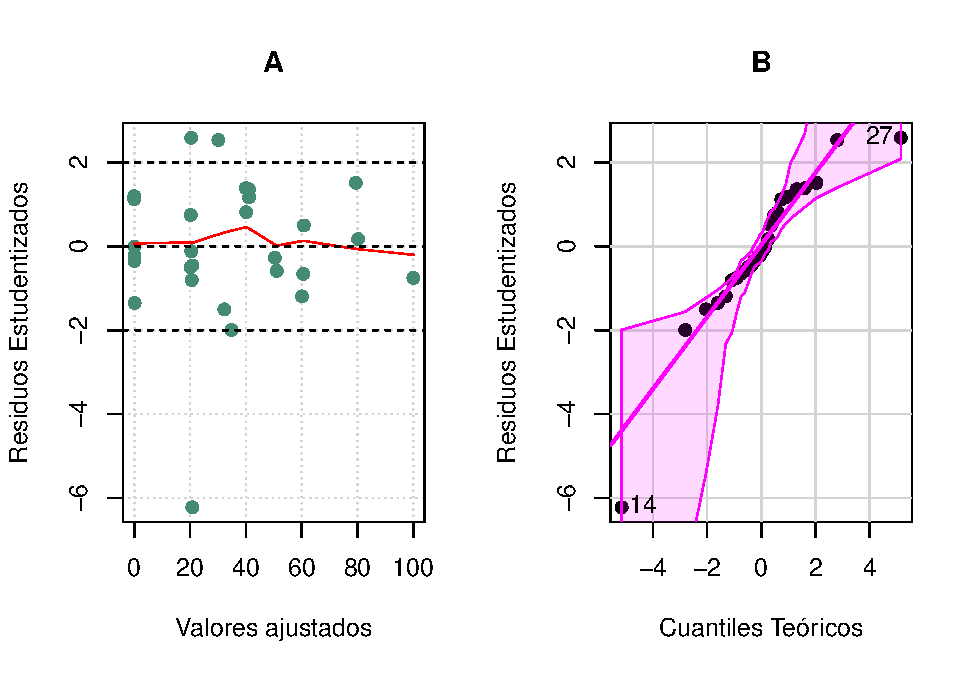
\includegraphics{Taller-2-Regresion-Multiple-Aplicada_files/figure-latex/unnamed-chunk-4-1.pdf}
{[}1{]} ``Shapiro Test''

\begin{verbatim}
Shapiro-Wilk normality test
\end{verbatim}

data: studres(model) W = 0.86458, p-value = 0.001868

{[}1{]} ``Breusch Pagan Test''

\begin{verbatim}
studentized Breusch-Pagan test
\end{verbatim}

data: model BP = 27.288, df = 24, p-value = 0.2912

Como no se cumple el supuesto de normalidad se procede a corregir
mediante el metodo de BoxCox y se verifica el cumplimiento de los
mismos.

\begin{Shaded}
\begin{Highlighting}[]
\NormalTok{model }\OtherTok{\textless{}{-}} \FunctionTok{lm}\NormalTok{(density}\FloatTok{+0.0000001} \SpecialCharTok{\textasciitilde{}}\NormalTok{ .}\SpecialCharTok{{-}}\NormalTok{NIR1}\SpecialCharTok{{-}}\NormalTok{NIR8}\SpecialCharTok{{-}}\NormalTok{NIR9}\SpecialCharTok{{-}}\NormalTok{NIR10}\SpecialCharTok{{-}}\NormalTok{NIR11}\SpecialCharTok{{-}}\NormalTok{NIR7, }\AttributeTok{data=}\NormalTok{X)}
\FunctionTok{lambda}\NormalTok{(model,}\SpecialCharTok{{-}}\DecValTok{3}\NormalTok{,}\DecValTok{3}\NormalTok{)}
\end{Highlighting}
\end{Shaded}

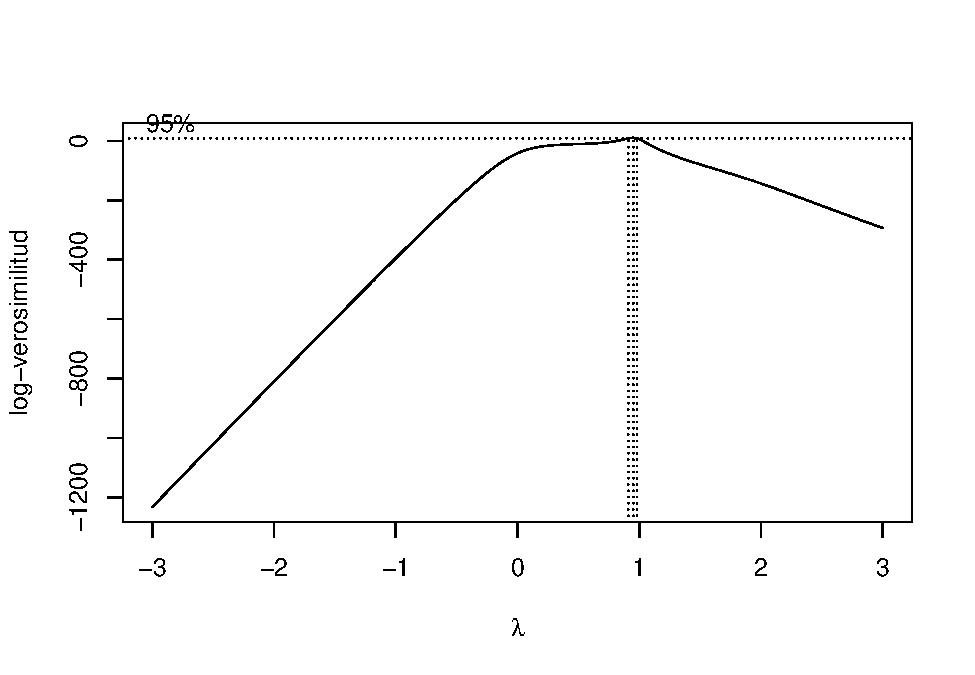
\includegraphics{Taller-2-Regresion-Multiple-Aplicada_files/figure-latex/unnamed-chunk-5-1.pdf}
{[}1{]} 0.95

\begin{Shaded}
\begin{Highlighting}[]
\NormalTok{model.box }\OtherTok{\textless{}{-}} \FunctionTok{lm}\NormalTok{(}\FunctionTok{I}\NormalTok{(density}\SpecialCharTok{\^{}}\FloatTok{0.95}\NormalTok{) }\SpecialCharTok{\textasciitilde{}}\NormalTok{.}\SpecialCharTok{{-}}\NormalTok{NIR1}\SpecialCharTok{{-}}\NormalTok{NIR8}\SpecialCharTok{{-}}\NormalTok{NIR9}\SpecialCharTok{{-}}\NormalTok{NIR10}\SpecialCharTok{{-}}\NormalTok{NIR11}\SpecialCharTok{{-}}\NormalTok{NIR7,}\AttributeTok{data=}\NormalTok{X)}
\FunctionTok{validaciongrafica}\NormalTok{(model.box)}
\end{Highlighting}
\end{Shaded}

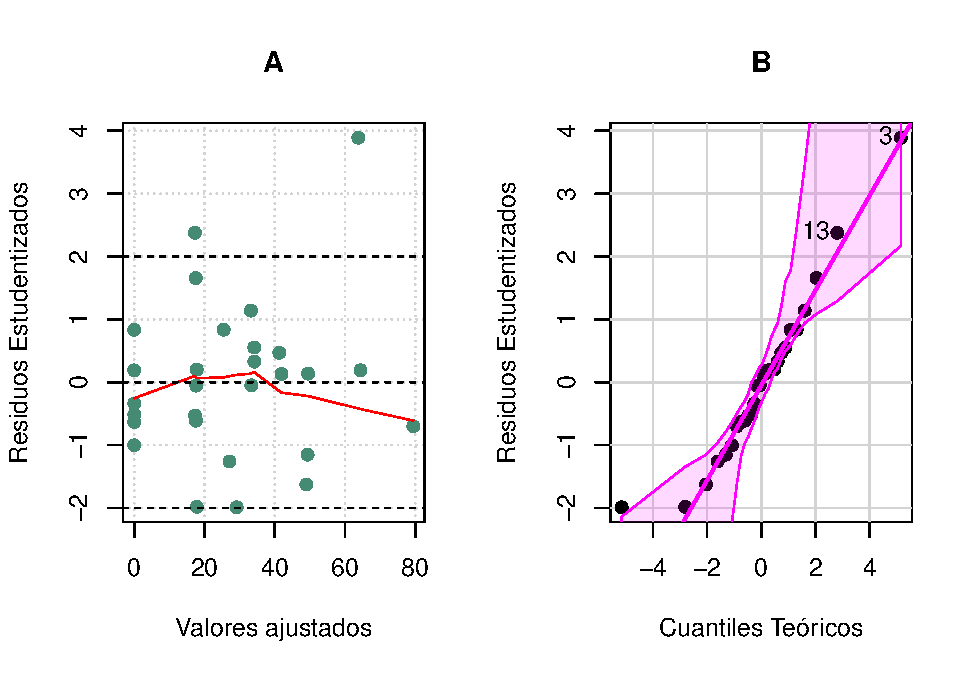
\includegraphics{Taller-2-Regresion-Multiple-Aplicada_files/figure-latex/unnamed-chunk-5-2.pdf}
{[}1{]} ``Shapiro Test''

\begin{verbatim}
Shapiro-Wilk normality test
\end{verbatim}

data: studres(model) W = 0.93504, p-value = 0.08267

{[}1{]} ``Breusch Pagan Test''

\begin{verbatim}
studentized Breusch-Pagan test
\end{verbatim}

data: model BP = 22.009, df = 24, p-value = 0.5787

\hypertarget{section}{%
\section{}\label{section}}

\begin{Shaded}
\begin{Highlighting}[]
\NormalTok{X.}\OtherTok{\textless{}{-}}\FunctionTok{model.matrix}\NormalTok{(model.box)[,}\SpecialCharTok{{-}}\DecValTok{1}\NormalTok{]}
\NormalTok{lasso.mod }\OtherTok{\textless{}{-}} \FunctionTok{glmnet}\NormalTok{(X., X}\SpecialCharTok{$}\NormalTok{density, }\AttributeTok{alpha =} \DecValTok{1}\NormalTok{,}\AttributeTok{nlambda =} \DecValTok{100}\NormalTok{)}
\NormalTok{lasso.mod}\SpecialCharTok{$}\NormalTok{beta}
\end{Highlighting}
\end{Shaded}

24 x 81 sparse Matrix of class ``dgCMatrix''

NIR2 . . . . . . . .\\
NIR3 . . . . . . . .\\
NIR4 . . 3.794159 12.13638 19.73747 26.66329 32.97384 38.72378 NIR5 . .
. . . . . .\\
NIR6 . . . . . . . .\\
NIR12 . . . . . . . .\\
NIR13 . . . . . . . .\\
NIR14 . . . . . . . .\\
NIR15 . . . . . . . .\\
NIR16 . . . . . . . .\\
NIR17 . . . . . . . .\\
NIR18 . . . . . . . .\\
NIR19 . . . . . . . .\\
NIR20 . . . . . . . .\\
NIR21 . . . . . . . .\\
NIR22 . . . . . . . .\\
NIR23 . . . . . . . .\\
NIR24 . . . . . . . .\\
NIR25 . . . . . . . .\\
NIR26 . . . . . . . .\\
NIR27 . . . . . . . .\\
NIR28 . . . . . . . .\\
NIR29 . -12.70035 -25.722352 -39.45434 -51.96639 -63.36691 -73.75464
-83.21956 NIR30 . . . . . . . .

NIR2 . . . . . .\\
NIR3 . . . . . .\\
NIR4 43.96291 48.73662 53.08623 57.04944 60.66057 61.276309 NIR5 . . . .
. 2.383012 NIR6 . . . . . .\\
NIR12 . . . . . .\\
NIR13 . . . . . .\\
NIR14 . . . . . .\\
NIR15 . . . . . .\\
NIR16 . . . . . .\\
NIR17 . . . . . .\\
NIR18 . . . . . .\\
NIR19 . . . . . .\\
NIR20 . . . . . .\\
NIR21 . . . . . .\\
NIR22 . . . . . .\\
NIR23 . . . . . .\\
NIR24 . . . . . .\\
NIR25 . . . . . .\\
NIR26 . . . . . .\\
NIR27 . . . . . .\\
NIR28 . . . . . .\\
NIR29 -91.84363 -99.70157 -106.86143 -113.38522 -119.32947 -125.150920
NIR30 . . . . . .

NIR2 . . . . . .\\
NIR3 . . . . . .\\
NIR4 47.80431 35.51972 24.32678 14.1290 4.83321 .\\
NIR5 16.84005 30.02088 42.03049 52.9725 62.94586 68.901969 NIR6 . . . .
. .\\
NIR12 . . . . . .\\
NIR13 . . . . . .\\
NIR14 . . . . . .\\
NIR15 . . . . . .\\
NIR16 . . . . . .\\
NIR17 . . . . . .\\
NIR18 . . . . . .\\
NIR19 . . . . . .\\
NIR20 . . . . . .\\
NIR21 . . . . . .\\
NIR22 . . . . . .\\
NIR23 . . . . . .\\
NIR24 . . . . . .\\
NIR25 . . . . . .\\
NIR26 . . . . . .\\
NIR27 . . . . . .\\
NIR28 . . . . . -1.143204 NIR29 -132.45140 -139.10460 -145.16671
-150.6902 -155.72346 -157.985303 NIR30 . . . . . .

NIR2 . . . . . .\\
NIR3 . . . . . .\\
NIR4 . . . . . .\\
NIR5 70.531043 72.015581 73.368727 74.601191 75.725100 76.74866 NIR6 . .
. . . .\\
NIR12 . . . . . .\\
NIR13 . . . . . .\\
NIR14 . . . . . .\\
NIR15 . . . . . .\\
NIR16 . . . . . .\\
NIR17 . . . . . .\\
NIR18 . . . . . .\\
NIR19 . . . . . .\\
NIR20 . . . . . .\\
NIR21 . . . . . .\\
NIR22 . . . . . .\\
NIR23 . . . . . .\\
NIR24 . . . . . .\\
NIR25 . . . . . .\\
NIR26 . . . . . .\\
NIR27 . . . . . .\\
NIR28 -2.921442 -4.596703 -6.142362 -7.565341 -8.866074 -10.05397 NIR29
-158.269644 -158.440388 -158.565340 -158.655379 -158.731275 -158.79575
NIR30 . . . . . .

NIR2 . . . . . .\\
NIR3 . . . . . .\\
NIR4 . . . . . .\\
NIR5 77.68023 78.53038 79.30481 80.01038 80.6532833 70.56035 NIR6 . . .
. 0.0204128 10.24270 NIR12 . . . . . .\\
NIR13 . . . . . .\\
NIR14 . . . . . .\\
NIR15 . . . . . .\\
NIR16 . . . . . .\\
NIR17 . . . . . .\\
NIR18 . . . . . .\\
NIR19 . . . . . .\\
NIR20 . . . . . .\\
NIR21 . . . . . .\\
NIR22 . . . . . .\\
NIR23 . . . . . .\\
NIR24 . . . . . .\\
NIR25 . . . . . .\\
NIR26 . . . . . .\\
NIR27 . . . . . .\\
NIR28 -11.14471 -12.14122 -13.05091 -13.88142 -14.6511081 -18.37418
NIR29 -158.84040 -158.87761 -158.90864 -158.93425 -158.9547926
-156.73818 NIR30 . . . . . .

NIR2 . . . . . .\\
NIR3 . . . . . .\\
NIR4 . . . . . .\\
NIR5 58.85184 47.89464 37.80761 28.58535 20.17108 12.47659 NIR6 21.95293
32.90195 42.97805 52.18939 60.59337 68.27726 NIR12 . . . . . .\\
NIR13 . . . . . .\\
NIR14 . . . . . .\\
NIR15 . . . . . .\\
NIR16 . . . . . .\\
NIR17 . . . . . .\\
NIR18 . . . . . .\\
NIR19 . . . . . .\\
NIR20 . . . . . .\\
NIR21 . . . . . .\\
NIR22 . . . . . .\\
NIR23 . . . . . .\\
NIR24 . . . . . .\\
NIR25 . . . . . .\\
NIR26 . . . . . .\\
NIR27 . . . . . .\\
NIR28 -24.50111 -31.04741 -37.35758 -43.22911 -48.62544 -53.57896 NIR29
-150.93409 -144.16955 -137.47679 -131.19056 -125.39106 -120.05476 NIR30
. . . . . .

NIR2 . . . . . .\\
NIR3 . . . . . .\\
NIR4 . . . . . .\\
NIR5 5.49677236 . . . . .\\
NIR6 75.24894784 81.206627 81.55788 81.997161 82.402227 82.773686 NIR12
. . . . . .\\
NIR13 . . . . . .\\
NIR14 . . . . . .\\
NIR15 . . . . . .\\
NIR16 . . . . . .\\
NIR17 . . . . . .\\
NIR18 -0.01083383 -1.114076 -1.29050 -1.783698 -2.245068 -2.670771 NIR19
. . . . . .\\
NIR20 . . . . . .\\
NIR21 . . . . . .\\
NIR22 . . . . . .\\
NIR23 . . . . . .\\
NIR24 . . . . . .\\
NIR25 . . . . . .\\
NIR26 . . . . . .\\
NIR27 . . . . . .\\
NIR28 -58.04613412 -59.239421 -59.38639 -59.090167 -58.898262 -58.803828
NIR29 -115.20362777 -109.944696 -109.44715 -108.078007 -106.647542
-105.189505 NIR30 . . . . . .

NIR2 -2.057910 -4.238154 -6.219898 -8.029589 -9.674628 -11.172907 NIR3 .
. . . . .\\
NIR4 . . . . . .\\
NIR5 . . . . . .\\
NIR6 83.999042 85.105944 86.109820 87.026117 87.859065 88.617692 NIR12 .
. . . . .\\
NIR13 . . . . . .\\
NIR14 . . . . . .\\
NIR15 . . . . . .\\
NIR16 . . . . . .\\
NIR17 . . . . . .\\
NIR18 -3.599762 -4.133950 -4.612239 -5.048334 -5.444251 -5.804728 NIR19
. . . . . .\\
NIR20 . . . . . .\\
NIR21 . . . . . .\\
NIR22 . . . . . .\\
NIR23 . . . . . .\\
NIR24 . . . . . .\\
NIR25 . . . . . .\\
NIR26 . . . . . .\\
NIR27 . . . . . .\\
NIR28 -62.446155 -66.845376 -70.849577 -74.534730 -77.862557 -80.890168
NIR29 -95.502717 -86.486263 -78.317767 -70.815154 -64.033565 -57.863003
NIR30 . . . . . .

NIR2 -12.539999 -13.785112 -14.917201 -15.949461 -16.888772 -17.746589
NIR3 . . . . . .\\
NIR4 . . . . . .\\
NIR5 . . . . . .\\
NIR6 89.309702 89.939815 90.512714 91.035070 91.510308 91.944262 NIR12 .
. . . . .\\
NIR13 . . . . . .\\
NIR14 . . . . . .\\
NIR15 . . . . . .\\
NIR16 . . . . . .\\
NIR17 . . . . . .\\
NIR18 -6.133354 -6.432135 -6.703404 -6.950788 -7.175475 -7.380793 NIR19
. . . . . .\\
NIR20 . . . . . .\\
NIR21 . . . . . .\\
NIR22 . . . . . .\\
NIR23 . . . . . .\\
NIR24 . . . . . .\\
NIR25 . . . . . .\\
NIR26 . . . . . .\\
NIR27 . . . . . .\\
NIR28 -83.666234 -86.193836 -88.478686 -90.566572 -92.460661 -94.202167
NIR29 -52.212069 -47.069192 -42.416792 -38.167106 -34.311616 -30.770853
NIR30 . . . . . .

NIR2 -18.52559217 -19.2443922 -19.9079914 -20.5168279 -21.078136
-21.592869 NIR3 . . . . . .\\
NIR4 . . . . . .\\
NIR5 . . . . . .\\
NIR6 92.33949368 92.7097147 93.0572965 93.3806451 93.682682 93.962531
NIR12 . . . . . .\\
NIR13 . . . . . .\\
NIR14 . . . . . .\\
NIR15 . . . . . .\\
NIR16 . . . . . .\\
NIR17 . . . . . .\\
NIR18 -7.56615357 -7.7374991 -7.8959371 -8.0414884 -8.176823 -8.301187
NIR19 . . . . . .\\
NIR20 . . . . . .\\
NIR21 . . . . . .\\
NIR22 . . . . . .\\
NIR23 . . . . . .\\
NIR24 . . . . . .\\
NIR25 . . . . . .\\
NIR26 . . . . . .\\
NIR27 -0.03041173 -0.1814426 -0.4469192 -0.7849073 -1.175805 -1.594745
NIR28 -95.71283100 -96.9067639 -97.7900178 -98.4218404 -98.868276
-99.166330 NIR29 -27.61048351 -24.7525255 -22.1967142 -19.9373827
-17.898761 -16.078501 NIR30 . . . . . .

NIR2 -22.069050 -22.500598 -22.896204748 -23.26949545 -2.360596e+01 NIR3
. . . . .\\
NIR4 . . . . .\\
NIR5 . . . . .\\
NIR6 94.224311 94.462780 94.683057646 94.90572794 9.510615e+01 NIR12 . .
. . .\\
NIR13 . . . . .\\
NIR14 . . . . .\\
NIR15 . . . . .\\
NIR16 . . . . .\\
NIR17 . . . . .\\
NIR18 -8.417521 -8.521819 -8.618090131 -8.71184840 -8.787072e+00 NIR19 .
. . . -1.148856e-04 NIR20 . . . . .\\
NIR21 . . . . .\\
NIR22 . . . . .\\
NIR23 . . . . .\\
NIR24 . . . . .\\
NIR25 . . . . .\\
NIR26 . . -0.002890285 -0.07992496 -1.894303e-01 NIR27 -2.039702
-2.473801 -2.900459262 -3.28638148 -3.598078e+00 NIR28 -99.355566
-99.453826 -99.486948183 -99.46891795 -9.941658e+01 NIR29 -14.404859
-12.946306 -11.629490931 -10.31627932 -9.217543e+00 NIR30 . . . . .

NIR2 -2.392113e+01 -2.421279e+01 -2.431158e+01 -2.426103e+01
-2.395712e+01 NIR3 . . -2.320394e-01 -5.644514e-01 -1.211884e+00 NIR4 .
. . . .\\
NIR5 . . . . .\\
NIR6 9.529872e+01 9.548073e+01 9.574040e+01 9.598956e+01 9.636566e+01
NIR12 . . . . .\\
NIR13 . . . . .\\
NIR14 . . . . .\\
NIR15 . . . . .\\
NIR16 . . . . .\\
NIR17 . . . . .\\
NIR18 -8.857794e+00 -8.923013e+00 -8.990648e+00 -9.037487e+00
-9.110196e+00 NIR19 -2.513917e-04 -3.704223e-04 -4.811274e-04
-5.381095e-04 -6.215297e-04 NIR20 . . . . -2.409418e-04 NIR21 .
-1.207928e-04 -1.106884e-03 -1.826650e-03 -2.333439e-03 NIR22
-1.143476e-03 -2.698802e-03 -3.222333e-03 -3.599785e-03 -4.025860e-03
NIR23 -1.905222e-04 -6.475062e-04 -1.085326e-03 -1.402280e-03
-1.757179e-03 NIR24 . . . . .\\
NIR25 . . . . .\\
NIR26 -3.314835e-01 -4.920745e-01 -6.978628e-01 -8.604441e-01
-1.142778e+00 NIR27 -3.866792e+00 -4.105796e+00 -4.328931e+00
-4.505309e+00 -4.695680e+00 NIR28 -9.933604e+01 -9.923442e+01
-9.910492e+01 -9.899506e+01 -9.881803e+01 NIR29 -8.188847e+00
-7.230282e+00 -6.270652e+00 -5.586568e+00 -4.628778e+00 NIR30 . . . . .

NIR2 -2.166155e+01 -16.41090910 -12.9064005 -9.7283402 -6.7176940 NIR3
-4.216273e+00 -10.12971709 -13.8758068 -17.2734601 -20.4907937 NIR4 . .
. . .\\
NIR5 . . . . .\\
NIR6 9.770773e+01 99.72205425 100.8879087 101.9515364 102.9628077 NIR12
. . . . .\\
NIR13 . . . . .\\
NIR14 . . . . .\\
NIR15 . . . . .\\
NIR16 . . . . .\\
NIR17 . . . . .\\
NIR18 -9.316036e+00 -9.26679283 -9.3509642 -9.4365081 -9.5143902 NIR19
-5.047180e-04 . . . .\\
NIR20 -2.016432e-04 . . . .\\
NIR21 -2.385099e-03 . . . .\\
NIR22 -4.099652e-03 -0.10431203 -0.1768564 -0.2518206 -0.3302481 NIR23
-1.408331e-02 -0.09810884 -0.1457378 -0.2024125 -0.2700970 NIR24 . . . .
.\\
NIR25 . . . . .\\
NIR26 -2.484058e+00 -3.66649572 -3.8395317 -3.9712904 -4.0926453 NIR27
-5.194754e+00 -5.76308641 -6.0528141 -6.2796102 -6.4676321 NIR28
-9.809083e+01 -96.78756675 -96.0300486 -95.3509070 -94.7110713 NIR29
-1.179934e+00 . . . .\\
NIR30 . . . . .

NIR2 -4.0582402 -1.4775166 . .\\
NIR3 -23.3393072 -25.9857596 -27.4644442 -2.750780e+01 NIR4 . -0.1725018
-0.3950726 -4.163678e-01 NIR5 . . . .\\
NIR6 103.8640898 104.8125286 105.4457504 1.054958e+02 NIR12 . . . .\\
NIR13 . . . .\\
NIR14 . . . .\\
NIR15 . . . .\\
NIR16 . . . .\\
NIR17 . . . -2.650788e-04 NIR18 -9.5805934 -9.6443366 -9.7010468
-9.706853e+00 NIR19 . . . .\\
NIR20 . . . .\\
NIR21 . . . .\\
NIR22 -0.4038774 -0.4765875 -0.5179921 -5.205979e-01 NIR23 -0.3413312
-0.4177564 -0.4645142 -4.677446e-01 NIR24 . . . .\\
NIR25 . . . .\\
NIR26 -4.1995439 -4.3079294 -4.4064034 -4.404672e+00 NIR27 -6.6145515
-6.7355174 -6.7208056 -6.727933e+00 NIR28 -94.1475808 -93.6219796
-93.3358281 -9.331713e+01 NIR29 . . . .\\
NIR30 . . . .

\begin{Shaded}
\begin{Highlighting}[]
\FunctionTok{plot}\NormalTok{(lasso.mod,}\AttributeTok{xvar=}\StringTok{\textquotesingle{}lambda\textquotesingle{}}\NormalTok{,}\AttributeTok{label=}\NormalTok{T,}\AttributeTok{lwd=}\DecValTok{2}\NormalTok{,}\AttributeTok{ylab=}\StringTok{\textquotesingle{}coeficientes de regresión\textquotesingle{}}\NormalTok{)}
\FunctionTok{abline}\NormalTok{(}\AttributeTok{h=}\DecValTok{0}\NormalTok{,}\AttributeTok{lty=}\DecValTok{2}\NormalTok{)}
\end{Highlighting}
\end{Shaded}

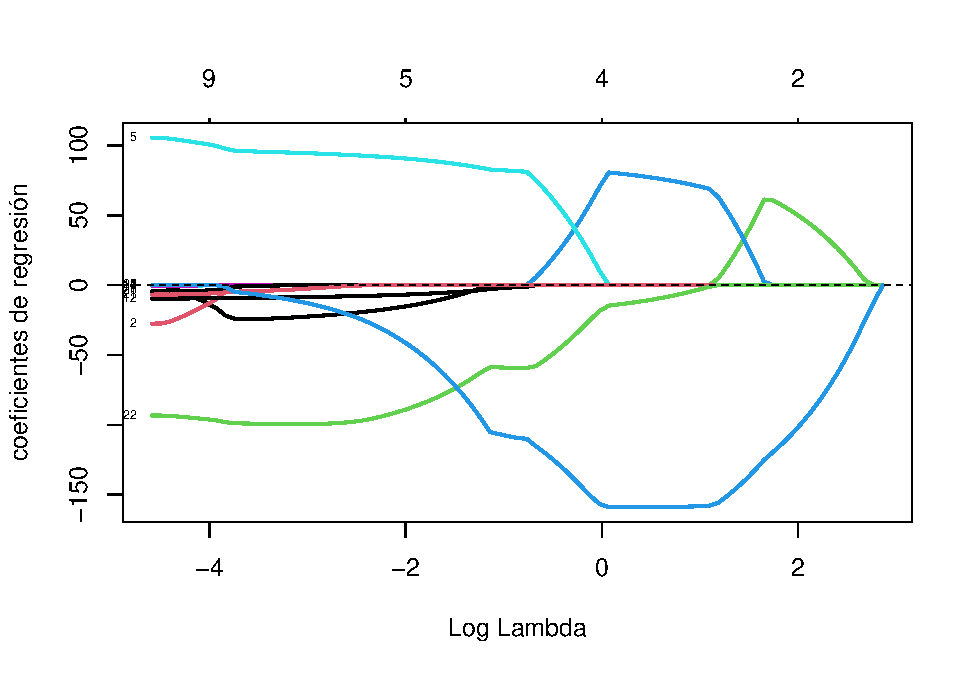
\includegraphics{Taller-2-Regresion-Multiple-Aplicada_files/figure-latex/unnamed-chunk-6-1.pdf}

\begin{Shaded}
\begin{Highlighting}[]
\NormalTok{lasso.cv }\OtherTok{\textless{}{-}}\FunctionTok{cv.glmnet}\NormalTok{(X., X}\SpecialCharTok{$}\NormalTok{density, }\AttributeTok{nfolds =} \DecValTok{4}\NormalTok{, }\AttributeTok{alpha =} \DecValTok{1}\NormalTok{,}\AttributeTok{nlambda =} \DecValTok{100}\NormalTok{)}
\FunctionTok{plot}\NormalTok{(lasso.cv)}
\end{Highlighting}
\end{Shaded}

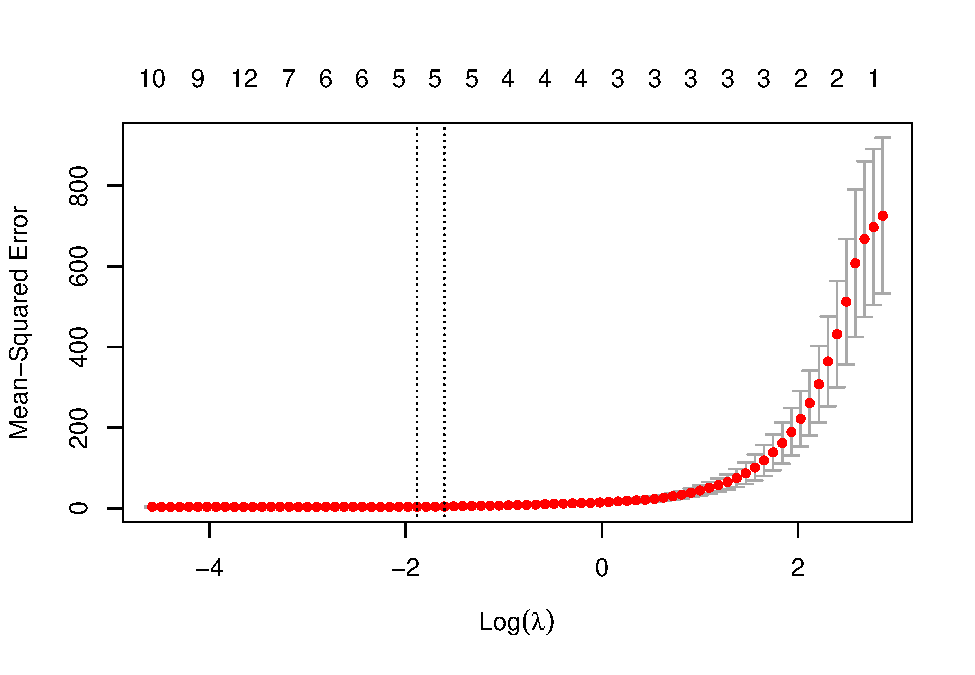
\includegraphics{Taller-2-Regresion-Multiple-Aplicada_files/figure-latex/unnamed-chunk-6-2.pdf}

\begin{Shaded}
\begin{Highlighting}[]
\NormalTok{est }\OtherTok{=} \FunctionTok{glmnet}\NormalTok{(X., X}\SpecialCharTok{$}\NormalTok{density, }\AttributeTok{alpha =} \DecValTok{1}\NormalTok{,}\AttributeTok{lambda =}\NormalTok{ lasso.cv}\SpecialCharTok{$}\NormalTok{lambda}\FloatTok{.1}\NormalTok{se)}
\NormalTok{est}\SpecialCharTok{$}\NormalTok{beta}
\end{Highlighting}
\end{Shaded}

24 x 1 sparse Matrix of class ``dgCMatrix'' s0 NIR2 -11.314302 NIR3 .\\
NIR4 .\\
NIR5 .\\
NIR6 88.544252 NIR12 .\\
NIR13 .\\
NIR14 .\\
NIR15 .\\
NIR16 .\\
NIR17 .\\
NIR18 -5.643411 NIR19 .\\
NIR20 .\\
NIR21 .\\
NIR22 .\\
NIR23 .\\
NIR24 .\\
NIR25 .\\
NIR26 .\\
NIR27 .\\
NIR28 -92.202115 NIR29 -40.266344 NIR30 .

\end{document}
